\documentclass[12pt letter]{report}
\input{../template/preamble}
\input{../template/macros}
\input{../template/letterfonts}

\usepackage{parskip}
\usepackage{tikz}
\usepackage{float}
\title{\Huge{Assignment 8}}
\author{\huge{Madiba Hudson-Quansah}}
\date{March 2024}


\begin{document}
\maketitle
\newpage

\qs{}{
  \begin{enumerate}
    \item do not contain the base T.
    \item contain the sequence ACG.
    \item contain all four bases A, T, C, and G.
    \item contain exactly three of the four bases A, T, C, and G.
  \end{enumerate}

}

\sol{

  \begin{enumerate}
    \item
          Using the restrictions given we are limited to the bases A, G and C for each position. This means there are
          three options for each position and since there are four positions we can split the task choosing a base
          into four steps, resulting in:
          \[
            3^4 = 81
          \]
          81 possible sequences.

    \item
          The sequence ACG is taken as a unit filling the first three positions from the left, allowing the remaining position to be filled
          with any if the four bases. Using the product rule this results in $4$ possible ways.\\

          But the unit ACG can also fill the first three positions from the right, which again only leaves one
          position left, using sum rule, this result in the total number of ways being:
          \[
            4 + 4 = 8
          \]
          8 possible ways
    \item
          The sequence must contain all for bases, this means that each of the four bases should appear once in the
          four element sequence, accounting for the order of appearance of all the bases being counted as a different
          sequence, we can use the permutation formula to calculate the total number of ways:
          \begin{align*}
            P \left( 4, 4 \right) & = \frac{4!}{(4 - 4)!} \\
                                  & = 24                  \\
          \end{align*}
          24 possible ways
    \item The sequence can contain exactly three of the four bases A, T, C, and G. This means that one of the bases
          must be left out, This leaves us with 3 possible bases to choose from for three of the four positions, and 3
          ways to choose the base to leave out. Using the product rule, we can calculate the total number of ways to
          choose a letter for each positions:
          \begin{align*}
            C \left( 4, 3 \right) \times C \left( 3, 1 \right) & = \frac{4!}{(4 - 3)!\times 3!} \times \frac{3!}{\left(
            3 - 1\right)! 1! }                                                                                          \\
                                                               & = 4 \times 3                                           \\
                                                               & = 12                                                   \\
          \end{align*}
          Now there are 4 possible positions to occupy with one of the bases as we have to choose exactly three out of four
          bases means exactly one base will be repeated out of the three bases chosen. This means that there are three
          possible positions to place the repeated base, giving us exactly 12 possible ways to choose the sequence. Using
          the product rule, then calculate the total number of ways adhere to the restrictions:
          \begin{align*}
            \text{Total number of ways to choose a letter} \times  \text{Number of ways to choose a sequence} & = 12 \times 12 \\
                                                                                                              & = 144          \\
          \end{align*}


  \end{enumerate}

}


\qs{}{
  What is the minimum number of students, each of whom comes from one of
  the 54 African countries, who must be enrolled at Ashesi university to guarantee that
  there are at least 5 who come from the same country? Explain.
}

\sol{
  Using the generalized pigeon-hole principle, the number of boxes $k$ is the number of African countries, $54$, and can
  represent the number of students needed to guarantee that there are at least 5 students from the same country, by $N$.
  Therefore:
  \begin{align*}
    \left\lceil \frac{N}{54} \right\rceil & = 5              \\
    4 < \frac{N}{54}                      & \leq 5           \\
    \\
    \frac{N}{54}                          & > 4              \\
    \frac{N}{54}                          & \leq 5           \\
    \\
    \frac{N}{54}                          & > 4              \\
    N                                     & > 216            \\
    \\
    \frac{N}{54}                          & \leq 5           \\
    N                                     & \leq 270         \\
    \\
    \\
                                          & 216 < N \leq 270
  \end{align*}
  $\therefore$ $N = 217$
}

\qs{}{
  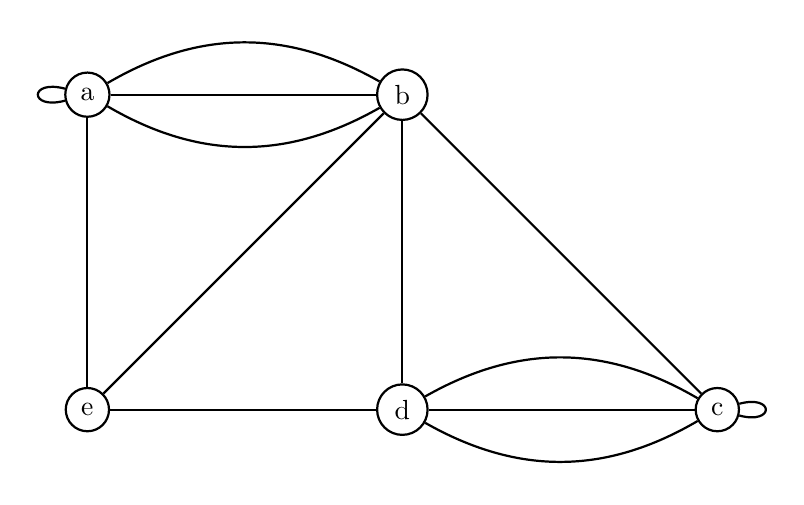
\begin{tikzpicture}[node distance={4cm}, thick, scale=0.5, main/.style = {draw, circle}]
    \tikzset{every loop/.style={}}
    \node[main] (1) {a};
    \node[main] (2)[right of=1] {b};
    \node[ main ] (3)[below of=1] {e};
    \node[ main ] (4)[right of=3] {d};
    \node[main](5)[right of=4] {c};
    \path
    (1) edge[loop left] (1)
    (1) edge (2)
    (1) edge[bend right] (2)
    (1) edge[bend left] (2)
    (1) edge (3)
    (2) edge(3)
    (2) edge (4)
    (2) edge (5)
    (3) edge (4)
    (4) edge[bend right] (5)
    (4) edge[bend left] (5)
    (4) edge (5)
    (5) edge[loop right] (5)
    ;
  \end{tikzpicture}
}

\sol{
  \begin{enumerate}
    \item
          There are 5 vertices, and 13 edges in the graph, with each vertex having a degree of:
          \begin{itemize}
            \item deg(a) - 6
            \item deg(b) - 6
            \item deg(c) - 6
            \item deg(d) - 5
            \item deg(e) - 3
          \end{itemize}
    \item Let $m$ be the number of edges, where $m = 13$.
          \begin{align*}
            2m                                                     & = \displaystyle\sum_{v \in V} \text{deg}\left( v \right) \\
            \\
            2m                                                     & = 26                                                     \\
            \displaystyle\sum_{v \in V} \text{deg}\left( v \right) & = 3 \left( 6 \right) + 5 + 3                             \\
                                                                   & = 26                                                     \\
            \frac{26}{2}                                           & = 13                                                     \\
          \end{align*}
  \end{enumerate}
}

\end{document}
